% The integer triangle P = conv((0,0),(2,0),(0,1)), whose long edge has slope -1/2,
% meets the box [-1,1]^2 in a polygon with the non-integral vertex (1,1/2).
\documentclass[border=2pt]{standalone}
\usepackage{tikz}
% Shared colours of the research figures (matplotlib tab10, as in the Berkovich skeleton figure).
\usepackage{amsmath}
\usetikzlibrary{calc}
\definecolor{figink}{HTML}{262626}
\definecolor{figred}{HTML}{D62728}
\definecolor{figblue}{HTML}{1F77B4}

\begin{document}
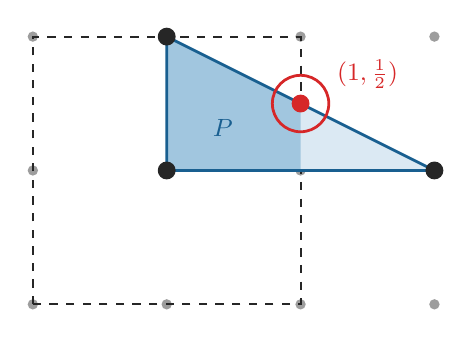
\begin{tikzpicture}[scale=1.7]
  % lattice points
  \foreach \x in {-1,...,2} \foreach \y in {-1,...,1}
    \fill[figink!45] (\x,\y) circle (1.1pt);
  % the box [-1,1]^2
  \draw[figink, line width=0.7pt, dashed] (-1,-1) rectangle (1,1);
  % the triangle P
  \fill[figblue!16] (0,0) -- (2,0) -- (0,1) -- cycle;
  % its intersection with the box
  \fill[figblue!42] (0,0) -- (1,0) -- (1,0.5) -- (0,1) -- cycle;
  \draw[figblue!80!black, line width=1pt, line join=round] (0,0) -- (2,0) -- (0,1) -- cycle;
  % integer vertices of P
  \foreach \v in {(0,0),(2,0),(0,1)}
    \fill[figink] \v circle (1.9pt);
  % the non-integral vertex of P cap box
  \fill[figred] (1,0.5) circle (1.9pt);
  \draw[figred, line width=1pt] (1,0.5) circle (6pt);
  \node[figblue!80!black, font=\small] at (0.42,0.32) {$P$};
  \node[figred, font=\small, anchor=west] at (1.2,0.72) {$(1,\tfrac12)$};
\end{tikzpicture}
\end{document}
